\documentclass{paper}

\usepackage{graphicx}
\usepackage{placeins}
\usepackage[utf8]{inputenc}
\usepackage{listings}
\usepackage{hyperref}
\usepackage{xcolor}

\definecolor{darkgreen}{RGB}{50,200,50}
\definecolor{verylightgray}{gray}{0.85}
\definecolor{goldenbrown}{rgb}{0.558215, 0.0, 0.135316}

\lstdefinelanguage{solidity}
{
	keywords={uint256, bytes32, mapping, address, uint40, bool, uint32, msg, sender, false, true},
	keywordstyle=\color{blue},
	keywords=[2]{pragma, contract, event, enum, struct, function, return, private, public, constant, returns, var, for, !, if, break, continue, throw, &&, ||, else, =, ==, <, >, <=, >=},
	keywordstyle=[2]\color{magenta},
	comment=[l]{//},
	commentstyle=\color{darkgreen},
	numbers=left,
	extendedchars=false,
	morestring=[b]",
	stringstyle=\color{goldenbrown},
	breaklines=true,
	backgroundcolor=\color{verylightgray},
	basicstyle=\linespread{1}\ttfamily\footnotesize
}

\title{Consensus in declarative process models using distributed smart-contracts}
\author{Mikkel Gaub, \\ Trondúr Høgnason, \\ Malthe Ettrup Kirkbro, \\ \& Mads Frederik Madsen }
\date{}

\begin{document}
	\begin{titlepage}
		\maketitle		
		\hspace{-18pt}
		\textit{May 15, 2017}
		\vspace{\fill}
		\section*{Abstract}
		This paper investigates how efficently declarative process models can be implemented using distributed smart-contracts, more concretely the Dynamic Condition Response (DCR) engine will be implemented on the Ethereum platform, with a focus on minimizing the cost of running such an engine.
		\thispagestyle{empty}
	\end{titlepage}
	\clearpage

	\pagenumbering{arabic}
	\setcounter{page}{1}

	\tableofcontents
	\pagebreak

	\section{Introduction}

	\section{DCR}

	Exclusion of Spawn relation.

	\section{Ethereum}

		\subsection{Blockchain}

		\subsection{Ethereum Virtual Machine}

		\subsection{Currency}

	\section{Implementation requirements}

	All of the proposed solutions will contain the following features:
	\begin{itemize}
		\item Creation of a workflow
		\item Execution of an activity
		\item Execution rights on the level of a user and on the level of a group
		\item Visibility?
	\end{itemize}


	\section{Multi-contract implementation}

	As the gas costs of ethereum are largely dominated by the price of creating a contract, creating a contract for each activity seems unfeasible and also has security concerns related to it which will be covered later...

	The first proposed solution is creating a contract for each workflow...

	\section{Mono-contract implementation}

	The second proposed solution is creating a single contract which controls all workflows...

	\section{Comparison}
	In order to compare the solutions to each other, a simple workflow has been created modelling each of the five relations...

	\begin{description}
		\item[Contract creation]
		\item[Successful execution] ...
		\item[Failed execution] ... 
	\end{description}

	\section{Optimizations}

		\subsection{Bitfields}

		\subsection{Incoming/Outgoing}

		\subsection{etc.}


	\section{Discussion}

	\section{Further features}

		\subsection{External relations}

		\subsection{Workflow changes}

		\subsection{External contract conditions}

	\section{Vulnerabilities}

		\subsection{External relations attack}

		\subsection{Workflow updating attack}

	\section{Conclusion}

	\pagebreak
	\addcontentsline{toc}{section}{References}	
	\begin{thebibliography}{99}

		\bibitem{test}
		Dr. Bib Example,
		\textit{How to bib},
		Penguin publishing,
		1994

	\end{thebibliography}

	\appendix

	\section{Gas prices}

		\begin{tabular}{| l | l |}
			\hline
			Action & Cost (gas) \\ \hline
			Contract creation & 0 \\
			\hline
		\end{tabular}

	\section{Test workflow}

		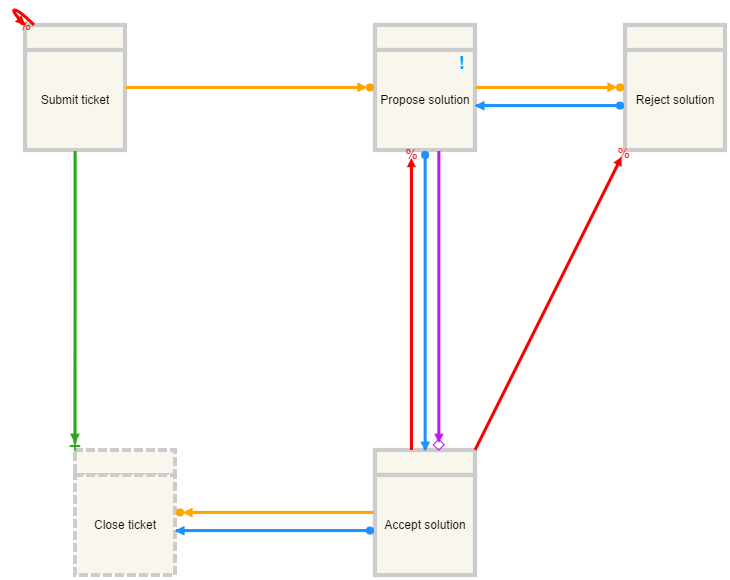
\includegraphics[scale=0.45]{figures/ExampleWorkflow.png}

	\section{Multi-contract}

		\subsection{Code}

			\lstinputlisting[language=solidity]{../contracts/workflow.sol}

		\subsection{Costs}

			\begin{tabular}{| l | l |}
				\hline
				Action & Cost (gas) \\ \hline
				Contract creation & 0 \\
				\hline
			\end{tabular}

	\section{Mono-contract}

		\subsection{Code}

			\lstinputlisting[language=solidity]{../contracts/monolith.sol}

		\subsection{Costs}

			\begin{tabular}{| l | l |}
				\hline
				Action & Cost (gas) \\ \hline
				Contract creation & 0 \\
				\hline
			\end{tabular}

\end{document}